%Delcare document type
\documentclass[]{article}

%Article information
\author{Justin Nicholson}
\date{\today}
\title{A Strategic Model of WTO Adjudication}

%Call nessecary external packages
\usepackage{multirow}
\usepackage{pdfpages}
\usepackage[margin=1in]{geometry}
\usepackage{caption}
\usepackage{setspace}
\usepackage{fancyhdr, amsmath, amssymb}
\usepackage{graphicx}
\usepackage{setspace}
\usepackage{hyperref}
\pagestyle{fancy}
\usepackage{spverbatim}
\usepackage{placeins}
\usepackage{amsthm}
%Fancy Header options
\lhead{Draft Paper}
\rhead{Nicholson}
\headheight = 14pt
\doublespace
\begin{document}
\maketitle
\section{introduction}
The budget for the World Trade Organization totaled roughly \$217,504,702.00 in 2013,the most recent year on record. There are currently 149 cases in consultations, including 4 in limbo since 1995. a further 43 cases are awaiting the composition or decision of a panel. This includes one case filed by the US against Argentina in 1999 over footwear and a Canadian case against the EEC over duties on imports of cereals. 160 states are members or observers, which accounts for roughly 82 percent of extant states. Adjudication, not to mention accession, is costly, often slow and bears no legal status beyond what the member states attribute to it. The question then is, why bother?  \\

In a world of complete information, we would expect bilateral bargaining to provide a resolution that is strictly Pareto superior to any resolution reached through a costly mechanism. Although Fearon discusses war, the logic goes through for any model where the alternative imposes a cost. Fairly standard reasoning then, would lead us to conclude that the the dispute settlement mechanism must impart some value over standard bargaining. Theories of adjudication often lead from the observation that democratic states utilize the mechanism more often than nondemocratic states. This has been explained through various incentives that democratic institutions create. Specifically, the three broad schools of thought conclude that the pressures of divided government, the incentives created by open elections or the values inherent in democratic systems are ultimately responsible for this empirical regularity. \\
 
\section{contribution}
This paper makes two broad contributions to the substantive literature on WTO adjudication by addressing two issues related by the presence of non-random action. The first issue is the data available for quantitative analysis. In her analysis of the democratic propensity to adjudicate, Christina Davis utilizes count data to model the propensity to adjudicate for WTO members. While useful, this exhibits a problematic yet subtle issue.  For $Y_{it}\geq 1$ observations in the data accurately reflect adjudicated cases, which necessarily implies a prima facie trade dispute exists. However, $Y_{it} = 0$ is a thornier issue. In fact in this case, it is not well defined. A zero may indicate that there were no potential trade disputes to adjudicate in a dyad year, or it may indicate that no dispute was selected for adjudication, however these are not equivalent if we wish to uncover the determinants of adjudication. One possible solution is the use of a Zero-Inflated Poisson model (ZIP), however with deeper data, we can directly study the initiation of adjudication from a set of \textit{potential} WTO disputes directly. \\

Event count models, and in particular ZIP/ZINB models mentioned above are abandoned because of the novel dataset constructed. However there are two interrelated reasons to abandon count models. First, we now have the flexibility to control for case-level factors to examine factors that affect the odds of filing, not just the propensity of a state to file, although the current availability of such data is admittedly sparse. However, it does allow for the model to take in to account the challenged state's decision to wait for a panel or not. We can therefore take into account the characteristic primacy of strategic interaction in the nature of international politics. Making use of the dispute settlement mechanism is not an automatic process that varies stochastically with exogenous regressors. The decision is made by an individual \footnote{While these decisions are often made by groups, the problem becomes almost completely intractable when viewed this way. Decisionmaking bodies and responsibilities vary wildly across states, most internal documents are not easily accessable etc. For the purposes of this paper, we will impose the unitary actor assumption standard in IR literature.}  in response to a choice problem. If this were a choice problem solved in a vacuum, then standard statistical models might still apply. In this case however, it is almost certainly the case that actions are chosen based on the expected probabilities over other players actions. In short, this is a problem of strategic action. Signorino and Yilmaz show that using a standard statistical model when strategic interaction is present is equivalent to accepting omitted variable bias " where the omitted variables are nonlinear higher-order terms associated with expected utility calculations" \cite{SY2003}. Using a non-strategic model can lead the analyst to directly opposite inferences than their strategic brethren when strategic interaction occurs. \\

Bearing this warning in mind, I offer an analysis utilizing strategic backwards induction on an improved dataset which contains the universe of potential disputes for a certain type of temporary trade barrier. Each observation is a potential Anti-Dumping trade dispute, whether or not it became a WTO dispute. The combination of data and method should allow for more precise results regarding the determinants of strategic interaction at the WTO. \\

 The bottom stage of the SBI model examines the determinants of panel formation once a dispute is filed. Keeping in mind that nearly 90\% of panel rulings favor the plaintiff, expected probabilities are derived. These probabilities are then included in a model of adjudication initiation with surprising and novel results. Both the model and the results will be discussed in more detail later in the article. 
\section{Theory}
While there have been a wide range of plausible theories put forward in regard to the use of the dispute mechanism of the WTO,  Christina Davis has convincingly argued that democracy is important above and beyond self-interested power politics.  This article does not mean to directly challenge that contention, but rather further explore \textit{how} democracy matters. At the risk of oversimplification, Davis posits that the institutions underpinning modern democratic states generate pressure to bring WTO disputes, in order to overcome a commitment problem.  In effect, the legislature induces this pressure by reducing the bargaining flexibility that the executive maintains, pushing them towards enforcement rather than bargaining. This implies a completely monotonic relationship: completely autocratic states feel no pressure to file at the WTO, beyond what might be considered rational self-interest, whilst extremely divided democracies or democracies experiencing divided government feel the most pressure to file.\\	

The analyses conducted thus far have have imposed the rather strong restriction of monotonicity on the regressors. \cite{SY2003}  I argue that this assumption is overly restrictive and unwarranted. Take for example Hein Goemans` hypothesis regarding international conflict. Goemans hypothesizes that ``Leaders of mixed regimes will suffer severe punishment whether they lose moderately or disastrously. Dictators and democrats are much more likely to suffer severe punishment when they lose disastrously than when they lose moderately" \cite{GGR2000}.  In a similar vein, I posit that \textit{mixed regimes} rather than strong democracies or strong autocracies have the most pressure to adjudicate at the WTO, ceterus paribus, and that in doing so they are in fact responding to incentives rationally. Repressive regimes have little incentive to utilize the WTO. They typically do not have liberal institutions that could put pressure on them, nor do they have a large electorate that they must please. These regimes need only please only a few select interests, and face little blowback on a case by case basis. Conversely, extremely open democratic regimes face large electorates with broad interests.\\ 

The contention that democratic regimes might prefer to be more reserved in their WTO filings might at first sound perverse, particularly so given that many of the states with the strongest democratic institutions were, and are, responsible for the primacy of the liberal-institutionalist trade regime.  Consider for a moment the problems that are encountered with pleasing large electorates. He might reason that the populace prefers a trade win, whether public or private over a trade loss in private, over a trade loss in public. With this preference ordering in mind, he might decide to bring only cases he knows he can win to the WTO, in order to win publicly and save more uncertain cases for other, more private venues where a loss can be swept under the electoral rug. 

 Perhaps the populace has a more consistent preference ordering, along the lines of. (insert here.), Even so, if It is now a long standing contention that  there is good reason to believe that the preferences indued by majority rule are not necessarily be coherent, and may indeed contain cycles. \cite{Arrow}. Riker shows that as the number of voters and issues grows large, we can expect quite large proportions of preference orderings without a Condorcet Winner. While this might seem abstract, it has practical implications for the political machinations a democratic leader. An unpopular decision now that comports with the leaders individual values regarding free trade in the present, does not preclude winning an election again in the future, holding other powerful governmental posts or a transition to the private sector. Further, some democracies employ term limits which free term-limited executives from electoral constraints beyond the control that loyalty and future patronage from their party induce.  

  Mixed regimes however face rather idiosyncratic restraints, and so their leaders must tread carefully. For an illustrative example, consider Pakistan. The state has alternated between periods of dictatorship and limited democracy, with non-transparent elections. A major electoral loss might result in the loss of power for many years, and exile or worse for the leaders of the former ruling party.  Making matters worse, the apparatus of repression is weaker than what a true despotic regime might be able to call upon, a la the East German Stazi. It might then be preferable for a leader to tie hands, and bring more cases before the WTO, preferring all cases to be handled publicly, and with the appearance that decisions are beyond their control. The clear case presented thus far is however muddled by the increased need to keep certain influential leaders happy. This might impart a desire to handle disputes quickly and efficiently. The same logic applies, however. By keeping the appearance of hands tied by international institutions and bringing all issues there, leaders can appear to be active in protecting interests, while avoiding the potential fallout from a private failure. 

 Note that the decisions above are all conditional on expected outcomes. The leader of a democracy for example will make his decision whether or not to escalate a case to the WTO based on his expectations over the outcome of the potential dispute, and that expected outcome's consequential effects on the political calculus. This implies the need to account for expectations over the actions of the other actors, who in turn are are making their own decisions based on their expectations. This implies that characteristics of the other defendant need to be accounted for explicitly both in the direct effect on the utility of the aggressor, and their indirect effect through the changes in his expected utility calculation, induced by the probability distribution over the defendants choices. 

In order to successfully account for the strategic nature of the situation, we must move beyond the traditional realm of binary or count based generalized linear models. Expectations over the actions implied by characteristics of the other actors need to be accounted for explicitly, and merely including more controls in a standard regression does not suffice. Instead, the strategic interaction models developed by Curt Signorino et al. are suited perfectly to this situation. However, this in turn implies the need for a new dataset, which contains deeper  data than is generally available. 

\section{new dataset}
Any quantitative analysis of the WTO dispute settlement mechanism will face some idiosyncratic challenges. The data ranks first and foremost among these issues.  In order to test the proposed theory with a method that adequately takes into consideration the concerns raised thus far,  we have need of a new data source. As mentioned in the introduction, most data available on this issue takes the form of count data. This type of data will not serve our purposes, since we need decision level data to feed our strategic model.   

\subsection{identifying potential cases}
One  of the signal issues in conducting this analysis is identifying the universe of cases that have the potential to become a WTO dispute. It is not immediately obvious what a potential case might be in general. However, We can narrow down the potential options by examining the subset of WTO cases that arise out of dumping / anti-dumping disputes. WTO rules allow a members state to identify and preliminarily address claims of market dumping. An investigation can result in either an anti-dumping action being taken over the potential trade barrier, or no action taken. The state targeted with the anti-dumping measure can then decide whether or not to escalate the dispute to a WTO adjudication case. If escalated, this case can be either be settled in the consultation phase, or continue on to panel formation. Panel formational overwhelming results in a ruling for the plaintiff. \\

The kernel of the dataset is derived from The Temporary Trade Barrier dataset, compiled by Chad Bowen. This dataset takes an investigation into a dumping violation as an observation. I take a potential WTO case as any observation that results in at least a preliminary anti-dumping action logged in the anti-dumping portion of The Temporary Trade Barrier Database, where both the investigated and the investigating states are WTO members. \cite{BADD}. This results in 1696 observations, from 1993 through 2012\footnote{All cases considered in this paper from the GATT period were adjudicated after the formation of the WTO.}, although several observations are subsequently dropped in the analysis section due to lack of information. Although there is good reason to assume that the missing data might not be random, there are so few observations compared to the rest of the data, that it is inconsequential. Further, some observations are not unique; i.e. some anti-dumping measures result in more than one WTO dispute. While examining what factor might lead to a multiple-filing at the WTO, we treat these cases as the same as single-filings. non-unique records are eliminated. 

\subsection{more about the data}
A WTO dispute is a dyadic relationship involving two parties and a time period. One state is the ``plaintiff" or sender, whilst the other state in the pair is the ``defendant" or target. The WTO does not actively enforce it`s rules, instead it relies on a ``fire alarm" type enforcement mechanism. States need to file disputes, and we take the result as a binary choice, i.e. 0 or 1. For the purposes of this analysis, third party interest in a case is ignored.  \\

Most problematic is the sparsity of data on what change, if any, triggered the investigation and similarly what change in anti-dumping measures, if any, triggered the WTO dispute. Although it might seem forced by the data, treating investigations as largely exogenous however is not as problematic as it might appear. This is a decision often undertaken by an autonomous or quasi-autonomous government division, and in regards to a relatively technical article of the WTO charter and it can be argued that there are easier articles to manipulate if a trumped up challenge is desired.  Although there are often ``selection problems all the way down" in International Relations, the new data provides a deeper, if narrower, picture of dispute initiation than most other datasets available. 

\subsubsection{a further caveat - naming issues}
The original dataset was often not consistent in the naming of states. For example, take the state formerly known as the Union of Soviet Socialist Republics. Depending on the time period, it is sometimes coded as the USSR, Russia, The Russian Federation etc. Every effort was made to inspect and standardize inconsistent naming for our analysis.  Given the size of the dataset however, it is not clear that every single observation was sufficiently corrected. The appendix contains more detailed information, and in the few cases a coding decision might be controversial, an explanation of the logic behind the coding choices. \\

For now, note that continuity is stressed; i.e. if a case was filed against the USSR and continued by Russia after the fall of the Soviet Union, then the data was coded to allow analysis of the case against that entity, no matter its name. Similarly, I assume that the unified post-1991 state of Germany properly inherited the disputes initiated by and targeted against the entity formerly known as The Federal Republic of Germany (i.e. West Germany).

\subsection{methods}
The data is first subjected to a traditional generalized linear model analysis. Following the specification and interpretation of several models of this type, the data is subjected to a series of strategic interaction models. Finally the results are then compared, and extensions are proposed. 

\section{empirical analysis}
\subsection{the dependent variable}
We will examine two dependent variables in our analysis. The first variable is \textit{challenge}, an indicator that takes the value 1 if a potential trade dispute between two states escalates to a challenge issued at the WTO. Some potential disputes result in more than one challenge at the WTO. Regardless, these disputes are collapsed into a single observation in the data. There are 124 observations that include a challenge, and 1512 that do not.  \\

The second dependent variable is \textit{panel}, an indicator variable that takes a value of 1 if a challenge at the WTO has escalated to the panel stage, whilst a 0 indicates that the case never made it to a panel, either because it has yet to be acted upon, or it was settled ``out of court". Unfortunately further disaggregation on this point has proven difficult. While the WTO has a ``model timeline", allowing approximately 18 months to resolve a dispute,  many cases have been on the books for significantly longer. There is an element of ``informal settlement"; i.e. some states agree to indefinitely table their disagreement without formally withdrawing the complaint. However, it is not immediately clear when this action is being taken, or when a case stalls for more innocent reasons.  This is a fruitful area for future research,  and might lend credence to an audience costs type explanation. Regardless, there are 103 cases that go to a panel, and 21 that do not. 

\subsection{variables of interest}
Level of democracy for a given dispute is the variable of interest for the theory posited above. How to include democracy in a quantitative model is a thorny issue, with no clear resolution.  For our purposes, and within the constraints of available data,  we will proxy democracy with polity2 score. The determinants of this score are however problematic. It would be ideal to include a variable to proxy the institutional control on the executive that democracy induces, but this is already included in the polity score.  

\subsection{control variables}
\subsubsection{Economic controls}
Regardless of political variables, there is good reason to expect that states with large economies that are heavily dependent on trade will file more WTO cases than those who do not exhibit those characteristics. Even if they file a smaller share of total cases, they may have more filings in absolute terms than a state that has a small, isolated economy. To control for these economic power and trade reliance arguments, control variables for GDP and trade as a percent of GDP are included. Dyadic trade flow is also of interest, but presents a thorny  problem. There is a significant correlation between net trade flows and the control on \% exports. This does not present a problem beyond interpretation of that variable under most conditions as long as it is a control, but makes it impossible to test whether it is a causal variable or explains the data better than other candidates.  

\subsection{Results}
\subsubsection{stategic model of liberal trade}
I take this as the base model for all that follows. This model shows the importance of democracy while controlling for GDP and export dependence. Crucially, the model takes level of democracy for both the challenger and the target into account for both stages of the game. The results of the base model are reported below. We see that in the bottom subgame, both the challenger's and the target's polity score are  significant. The results indicate that the higher either polity score, the more likely it is that a defendant will hold out for a panel ruling in a given dispute, holding all else constant. However, the strategic model shows us that when the challenger takes this into consideration along with the specified independent variables, an increase in challenger polity score decreases the utility of challenging, ceterus paribus. To better see the result, I provide plotted predicted probabilities below. All variables are held at their mean, save challenger polity, which is allowed to vary. Note also that the y-axis is the probability of \textit{not challenging} or, equivalently, choosing the status quo.

The graph clearly shows the posited relationship exists, within the confines of this model. At the far left, where polity is near its` lower bound, the probability of not challenging is near 1. The probability decreases as polity increases, reaching a nadir around a score of 4, which corresponds to a mixed regime type. The probability then begins increasing again, ultimately approaching \%95, as polity reaches its maximum. 

\begin{table}[Htbp] \centering 
  \caption{Depdendent Variables} 
  \label{} 
\begin{tabular}{@{\extracolsep{5pt}}lccccc} 
\\[-1.8ex]\hline \\[-1.8ex] 
Statistic & \multicolumn{1}{c}{N} & \multicolumn{1}{c}{Mean} & \multicolumn{1}{c}{St. Dev.} & \multicolumn{1}{c}{Min} & \multicolumn{1}{c}{Max} \\ 
\hline \\[-1.8ex] 
chal & 1636 & 0.076 & 0.265 & 0 & 1 \\ 
panel.i & 1636 & 0.063 & 0.243 & 0 & 1 \\ 
\hline \\[-1.8ex] 
\end{tabular} 
\end{table} 

\subsection{standard probit analysis}
The first model run is a standard probit analysis of the new data, derived from the theory presented above. The dependent variable is \textit{challenge}, and the independent variables include economic controls and polity scores. The results are presented in table \ref{base logit} below. We see that challenger GDP is extremely significant, as is the target's polity score. All else equal, it appears that the more democratic you are, the more likely you are to be challenged. This is prima facie evidence for the theory put forward by Davis, that democracies prefer being challenged.  

\begin{table}[htbp] \centering 
  \caption{probit model of liberal trade} 
  \label{base probit} 
\begin{tabular}{@{\extracolsep{5pt}}lc} 
\\[-1.8ex]\hline \\[-1.8ex] 
\\[-1.8ex] & \textbf{chal} \\ 
\hline \\[-1.8ex] 
 polity, challenger\_IMP & 0.008 \\ 
  & (0.007) \\ 
  polity, target\_IMP & 0.061$^{***}$ \\ 
  & (0.015) \\ 
  GDP, challenger\_IMP & 0.173$^{***}$ \\ 
  & (0.037) \\ 
  trade \% GDP, challenger\_IMP & $-$0.0004 \\ 
  & (0.001) \\ 
  Constant & $-$6.730$^{***}$ \\ 
  & (1.120) \\ 
 N & 1624 \\ 
Log Likelihood & $-$413.921 \\ 
AIC & 837.842 \\ 
\hline \\[-1.8ex] 
\multicolumn{2}{l}{$^{***}$p $<$ .01; $^{**}$p $<$ .05; $^{*}$p $<$ .1} \\ 
\end{tabular} 
\end{table} 
\subsection{SBI analysis}
\begin{table}[p]
\begin{center}
\begin{tabular}{lcccc}
\hline
 & u1(\textasciitilde{}challenge) & u1(chal,\textasciitilde{}panel) & u1(challenge,panel) & u2(challenge,panel) \\
\hline
\multirow{2}{*}{(Intercept)} & \multirow{2}{*}{} & $-$28.3658875 & $-$2.3424977 & $-$1.1352196 \\
 &  & (9.7883254) & (2.8161675) & (0.9663111) \\[2pt]
\multirow{2}{*}{polity2, challenger} & 0.4385588 & \multirow{2}{*}{} & \multirow{2}{*}{} & 0.1035897 \\
 & (0.1289792) &  &  & (0.0200617) \\[2pt]
\multirow{2}{*}{polity2, target} & 0.0837155 & \multirow{2}{*}{} & \multirow{2}{*}{} & 0.0414620 \\
 & (0.0868104) &  &  & (0.0179849) \\[2pt]
\multirow{2}{*}{log GDP, challenger} & $-$0.2488223 & \multirow{2}{*}{} & \multirow{2}{*}{} & \multirow{2}{*}{} \\
 & (0.0628849) &  &  &  \\[2pt]
\multirow{2}{*}{\% trade of GDP, challenger} & 0.0021108 & \multirow{2}{*}{} & \multirow{2}{*}{} & \multirow{2}{*}{} \\
 & (0.0017180) &  &  &  \\[2pt]
\multirow{2}{*}{log GDP, challenger, target} & \multirow{2}{*}{} & \multirow{2}{*}{} & \multirow{2}{*}{} & 0.0789771 \\
 &  &  &  & (0.0347653) \\[2pt]
\multirow{2}{*}{log GDP, target} & \multirow{2}{*}{} & \multirow{2}{*}{} & \multirow{2}{*}{} & $-$0.0048068 \\
 &  &  &  & (0.0031106) \\[2pt]
\hline \hline
Log-likelihood & $-$412.499 \\
 $N$ & 1624\\
\hline
\end{tabular}
\end{center}
\caption{Strategic Model of Liberal Trade}
\label{tab:libtr}
\end{table}


\begin{table}[htbp]
\begin{center}
\begin{tabular}{lcccc}
\hline
 & u1(\textasciitilde{}chal) & u1(chal,\textasciitilde{}panel.i) & u1(chal,panel.i) & u2(chal,panel.i) \\
\hline
\multirow{2}{*}{(Intercept)} & \multirow{2}{*}{} & $-$29.5752389 & $-$2.5112022 & $-$1.2550877 \\
 &  & (10.9380864) & (2.9159430) & (1.8009770) \\[2pt]
\multirow{2}{*}{polity2, challenger} & 0.4374113 & \multirow{2}{*}{} & \multirow{2}{*}{} & 0.1034534 \\
 & (0.1421695) &  &  & (0.0295974) \\[2pt]
\multirow{2}{*}{polity2, challenger, target} & 0.0876272 & \multirow{2}{*}{} & \multirow{2}{*}{} & 0.0430477 \\
 & (0.0857358) &  &  & (0.0259945) \\[2pt]
\multirow{2}{*}{log GDP, challenger\_IMP} & $-$0.2545448 & \multirow{2}{*}{} & \multirow{2}{*}{} & \multirow{2}{*}{} \\
 & (0.0694800) &  &  &  \\[2pt]
\multirow{2}{*}{\% trade of GDP, challenger} & 0.0021335 & \multirow{2}{*}{} & \multirow{2}{*}{} & \multirow{2}{*}{} \\
 & (0.0019540) &  &  &  \\[2pt]
\multirow{2}{*}{log GDP, target\_IMP} & \multirow{2}{*}{} & \multirow{2}{*}{} & \multirow{2}{*}{} & 0.0842196 \\
 &  &  &  & (0.0672745) \\[2pt]
\multirow{2}{*}{\% trade of GDP, target} & \multirow{2}{*}{} & \multirow{2}{*}{} & \multirow{2}{*}{} & $-$0.0053112 \\
 &  &  &  & (0.0066016) \\[2pt]
\hline \hline
Log-likelihood & $-$414.0054755 \\
 $N$ & 1624\\
\hline
\end{tabular}
\end{center}
\caption{Trembling Hand Model of Liberal Trade}
\label{tab:libtrt}
\end{table}


Of course, these models would not be of much interest to us if they were incomparable. Since neither model can be expressed as a restriction of the other, a non-nested model test can be employed. Vuong test returns a test statistic of 3.1, indicating (p = 0.0021 that our strategic model performs significantly better than the non-strategic probit. A Clarke test is a bit murkier, giving no clear indication of which model is preferred. This is fairly strong evidence that the strategic model outperforms current methods, especially given that the the baseline strategic model fits 11 parameters, while the probit model fits only 5.  

We are also in a position to test some assumptions about the information structure of the model. Thus far, we have assumed that the source of variation is a probability distribution over private information, which implies that our model essentially produces a variant of a subgame perfect Nash equilibrium. We can depart form this assumption, and consequently the assumption of perfect rationality by assuming that the variation results from a ``trembling hand" or agent error. This type of model assumes that people can and do make mistakes. Table \ref{tab:libtrt} reports the results of a suitably modified strategic model. 

Both Clarke and Vuong test indicate that the private information model is preferred to the agent error model. However, there is still good substantive reason to believe that experience might play a factor in who files. Future research will include applying this model to only the subset of developing members of the WTO data developed Davis and Bermeo.  They argue that experience increases the likelihood of filing and there is  evidence from this model that  democracy is more important in an agent error model. Note that more both polity scores (for challenger and target) are more significant in the agent error models. Figure \ref{fig:predprobs} shows the predicted probabilities of both models side by side. While the two graphs are largely identical, the trembling hand model has a slightly larger minimum. \footnote{The minimum predicted value for the trembling hand model is 0.820 while the private information model has a minimum of 0.823. Note that this is the probability of \textit{not challenging}. More concrete evidence would be a more significant difference between models when restricted to \textit{non-sophisticated} members.}   If we take the small step of assuming that agent error primarily results from a lack of experience,  then the informal model comparison provides  circumstantial evidence for the logic of Davis and Bermeo`s argument, insofar as mixed regime states will be less likely to file when agent error is the correct information structure.

\begin{figure}[h]
   \centering
   \begin{tabular}{@{}c@{\hspace{.5cm}}c@{}}
       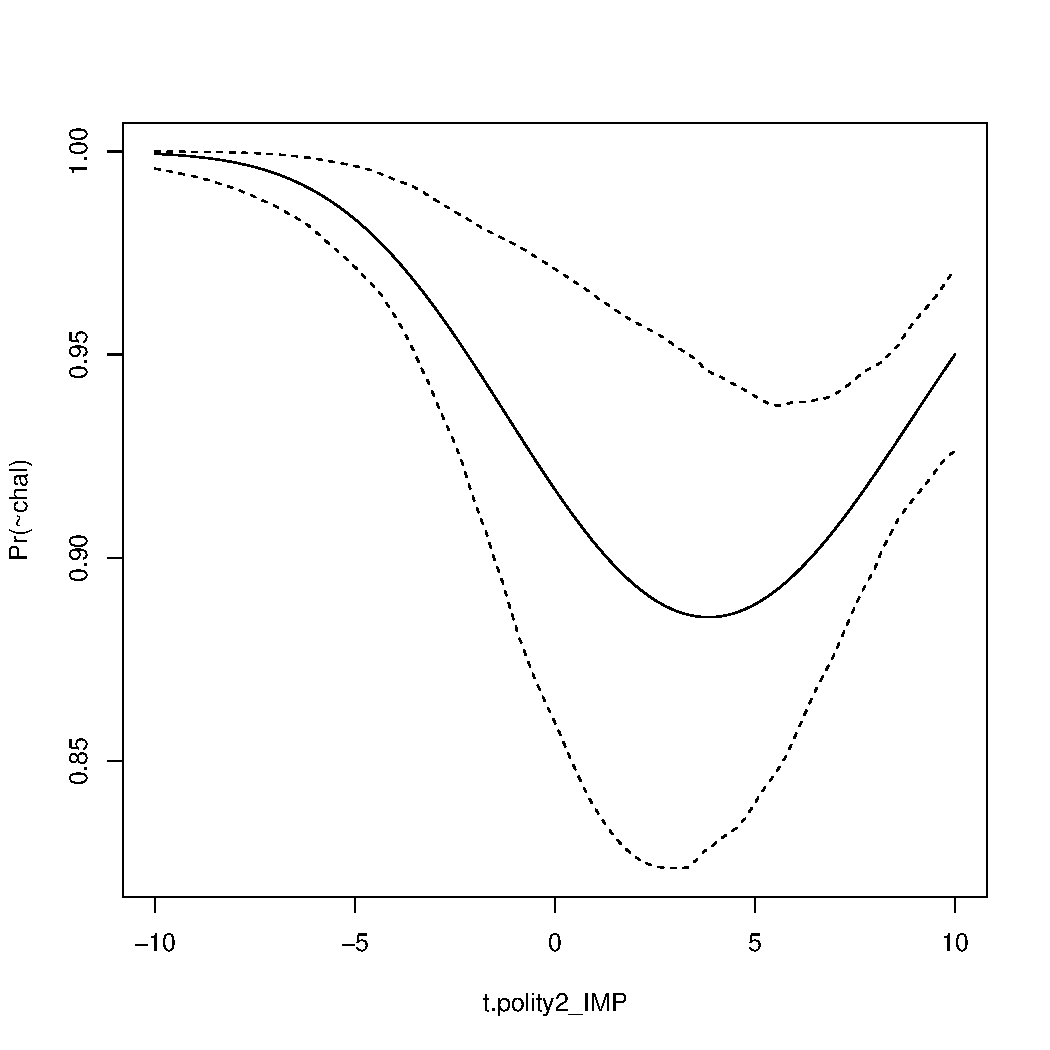
\includegraphics[page=1,width=.45\textwidth]{probs_tremble.pdf} & 
       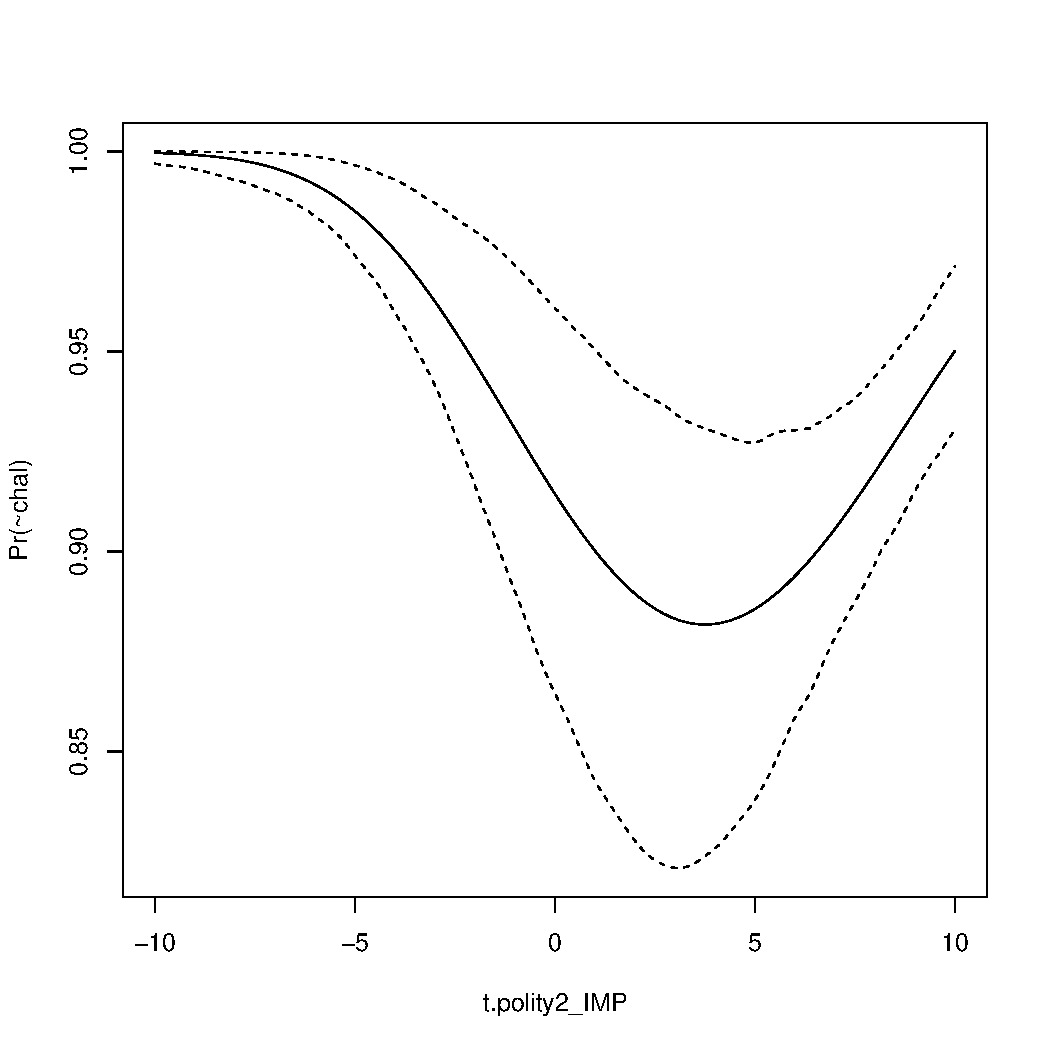
\includegraphics[page=1,width=.45\textwidth]{predplot1.pdf} \\[.5cm]\\
   \end{tabular}
 \caption{Predicted Probabilities\\ Trembling hand (L), Private Information (R)}
 \label{fig:predprobs}
\end{figure}
\section{conclusion}
\section{extensions}
%The observation that there are more WTO disputes filed by democracies, does not necessarily imply that WTO violations against democracies are more likely to be brought to the WTO.

\newpage
\bibliography{2yp}
\nocite{*}
\bibliographystyle{plain}
\end{document}